\chapter{Results and Discussion}

\section{Piezo1 as integrator of biomechanical events in MSCs}
\label{sec:piezo1-as-integrator-of-biomechanical-events-in-mscs}

\myworries{How does the peak relate to flow rate? Is there saturation?}
It is well known, that stem cell migration, differentiation and self-renewal is significantly influenced by physical interaction between the cell, its surrounding microenvironment and exogenous forces. \cite{Eyckmans2011, Lee2011}]MSCs are arguably the most thoroughly studied type of stem cell in this context, possibly because of the promising potential they hold for regenerative medicine and relative ease of access. Extensive studies of different force parameters (e.g. type, amplitude, static/dynamic) on MSCs give great insight into downstream pathways involved that guide the cells behaviour. However, the significance of \Piezo{} and the associated calcium-ion influx in MSC mechanosensing is not fully understood. In the following part we want to elucidate whether \Piezo{} is functionally able to elicit a significant intracellular signal in MSCs that can be classified as mechanotransductory significant.\\
In a reductionist approach, we conclude a relevant contribution of \Piezo{} given MSCs exhibit a \Piezo{}-mediated influx of extracellular calcium ions in response to force. \\
For our first experiment, Flowchambers were prepared with wild-type (WT) cells being seeded and stained as described in \vref{sec:FluidicModel}. For each flowchamber two separate calcium imaging recordings were carried out in close temporal sequence to each other: The first recording was done using the previously mentioned flow rate protocol executed with modified, calcium-free ACSF as flow shear medium. Upon completion of the first recording, the flow shear medium is exchanged for normal, calcium containing ACSF and the cells continuously flushed for 12 minutes with a total volume of 2.4 ml. After the flushing period, a second recording was done with the previously used flow rate protocol but this time with normal ACSF. After both measurements were completed, the integrity of the flowchamber was assessed by eye and the recordings deemed qualified for analysis, when no violation of structural integrity was observed. The sequence of first calcium-free and second calcium-containing medium is important, as reactive capability of the cells has to be demonstrated in the last measurement to rule out cell death as a possible explanation for lack of impulse response. We then concatenated the two measurements and let them \myworries{!finish at home, explain code pipeline}. We saw a maximum increase of up to 80\% in fluorescence signal in direct response to shear pulse as opposed to no or slightly negative pulse response in the calcium-free measurement. While the amplitude is likely a function of intracellular state, laminar flow defects and flowchamber and grating specific random errors, thus varying over different biological donors, we still see a clear-cut necessity of extracellular calcium-ion presence for successful impulse response. Surprisingly, the shear flow pulse seems to have a negative effect on fluorescence levels of the cell, as illustrated by the bump \myworries{Fig Reference}. We argue that this is likely a technical issue resulting from a combination of loosely-adherent highly fluorescent particles segmented as a cell and the static nature of our segmentation method. During the flow pulse, the particles are swept away, leaving only non-fluorescent substrate and thus leading to an incorrect classification of a decrease in fluorescence. A second technical issue is the discontinuity in apparent fluorescence between the two measurement, with the second measurement starting shy above a ratio of one. We argue this is due to the calcium-starved cell increasing the calcium-influx after resupplying them with extracellular calcium-ions during the flushing period. As this bias corresponds to maximally \myworries{XX}\% of the fluorescence response, we did not correct for this error. Another minor technicality is the slightly negative slope of the baseline. This corresponds to the known property of fluorescent markers to decrease in fluorescence as a function of light exposure, and is called Photobleaching. As the effect is likely neglibible, it is still important to keep in mind, that the signal in the second measurement likely would be slightly higher, since it has the added effect from the first measurement's photobleaching.

\begin{figure}
\centering
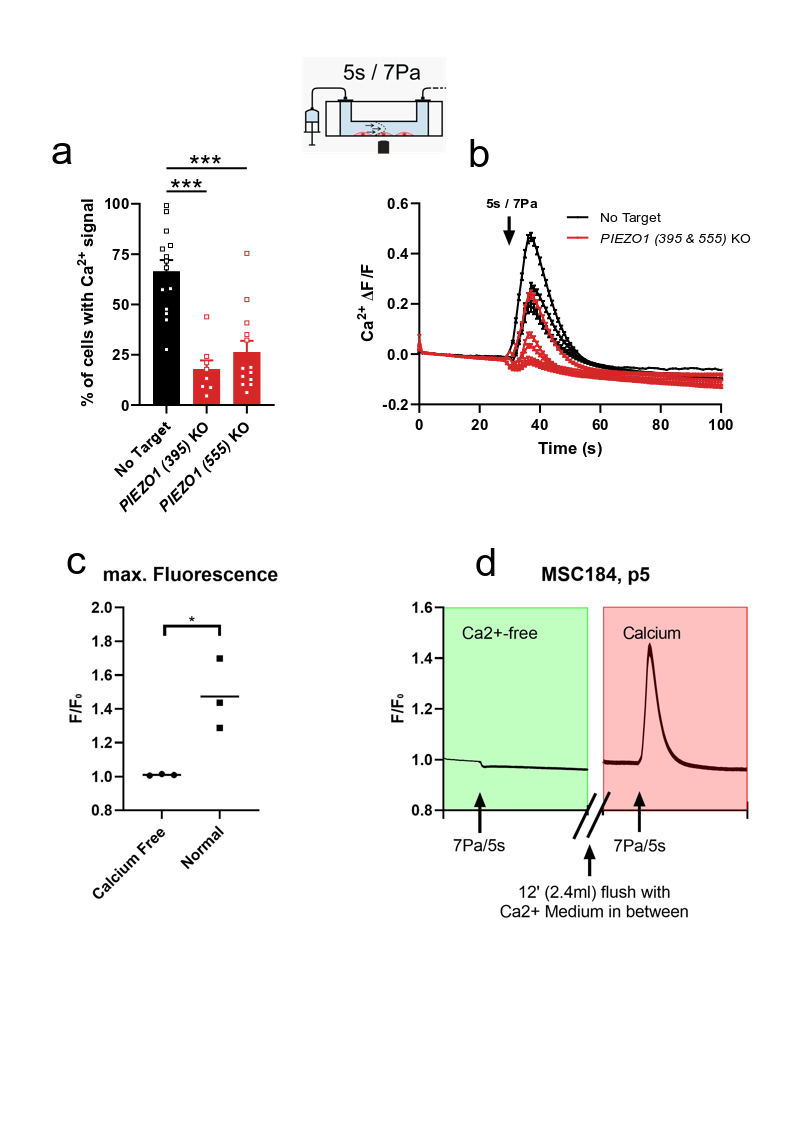
\includegraphics[width = 0.7\textwidth]{Combined_CalciumFree_KnockOut.png}
\caption{Piezo1-mediated influx of extracellular Ca2+ confirmed as mechanotransductory event in MSC. \hfill \newline 
\textbf{a.)} Representative fluorescence level measurement of impulse response with two different media where arrows mark the start of a 7Pa shear stress period of 5s. (Pooled data of 4 technical replicates, Data is mean $\pm$ SEM)	
\textbf{b.)} Peak values of fluorescence levels of samples in calcium-free and calcium-containing medium. (n = 3, *p $<$ 0.05, Student's t-test) 
\textbf{c.)} Temporally resolved fluorescence Signal of Piezo1-KO Cells compared to Control in response to 7 Pa shear period of 5s as denoted by arrow.  
\textbf{d.)} Relative amount of cells that showed fluorescence level impulse response. (Data points describe technical replicates, ***p$<$0.0001, ANOVA with Dunnette's multiple comparison test)}
\label{fig:CalcImaging_Cells}
\end{figure}

We demonstrated that MSCs exhibit reactive mechanosensitive capabilities through force-mediated rapid onset influx of extracellular calcium-ions. The role of \Piezo{} in this process, however, is not defined. To shed light on the contribution size of \Piezo{} we compared the impulse response capabilities of two distinct \Piezo{}-knock out constructs to a control cell line.\\
In preparation for this experiment three transfected cell lines were generated (2 distinct \Piezo{} knock-out's and one negative control) using pre-made lentivirus, carrying a CRISPR/Cas9-system with puromycin resistance as the selection marker. The grouping is specified through the Lentiviral Construct used, resulting in cell line P1-395 (Deletion at \myworries{Ask MATTHIAS}), P1-555 and NoT (No Target, Control for the viral treatment with no putative genome mutation).  In order to assess knock-out efficiency, both Western Blot and qRT-PCR were done not more than one passage after thawing, to avoid overestimation of knock-out efficiency as it likely increases with growing passages. With an knockout efficiency on mRNA-level of XX\% in P1-395 and XX\% in P1-555 and a corresponding knockout-efficiency on protein-level of XX\% in P1-395 and XX\% in P1-555, respectively, we can consider this cell line a valid knock-out model. \myworries{Add efficiency numbers of knockout} 

We then seeded cells in flowchambers and measured the intracellular calcium signal of the cells in response to a shear pulse, similar to the protocol from the previous experiment but only with a single measurement per flowchamber with normal ACSF as shear flow medium. Intriguingly, the knock-out cells show a significantly reduced reaction capability when compared to control. \myworries{FigReference} When comparing the relative amount of knock-out cells that exhibit calcium-influx in response to shear stress, we see a 66\% decrease compared to control, with the effect being bigger in P1-395 (-73\%) as in P1-555 (-60\%). Interestingly, this difference between two different constructs regarding their reduction of impulse response correlates with the knock-out efficiency. Figure 3.b, which shows the same data, but over full temporal resolution, illustrates how the area under the curve is largely reduced when \Piezo{} is knocked out. Modelling of the channel dynamics using a simple statistical model shows that, the decay mechanics largely stay the same with only the amplitude changing to lead to this result, or differently put: The model suggests that there is no compensating adaptation of single channel mechanics in response to lower channel abundance.

These results confirm that \Piezo{} is the main driver in force-mediated calcium-influx in mesenchymal stem cells.


\section{Piezo1 and the extracellular matrix}

Preliminary mass spectroscopy secretome analysis of \Yoda-treated cells showed a distinct decrease in core extracellular matrix (ECM) components, such as alpha-1 type I collagen (\colone), Fibronectin-1 (\textsc{Fn1}) and finally alpha-1 type III collagen (\colthree) (Not shown here).
This inspired further investigation into this matter.\par

After seeding cells in serum-free medium and letting them rest, we chemically stimulated \Piezo{} with \Yoda{} during 30 minutes, before washing them and transferring them in the incubator again, following the protocol described earlier \myworries{REF}. We then harvested identical samples right after intervention (d0) and after 24, 48 and 72 hours (denoted d1, d2 and d3, respectively) to achieve temporal resolution. Western Blot of intracellular protein showed a distinct decline in \colone in samples that have been treated with \Yoda{}. \myworries{FigureRef} Furthermore, the effects were not only marked by fast onset but also of long-lasting nature, since the effect of a singular 30 minutes \Yoda{}-exposition remained the same three days after intervention.\par
We also looked at mRNA representation of identical samples through qRT-PCR, with investigated mRNA's including \colone{}, \colthree{}, \textsc{Fn}1 and Interleukin-6 (IL-6) with GAPDH and RPL13A as house-keeping genes to confirm our prior results.  All measurements were normalised against negative control samples harvested immediately after the intervention.\\
While we were not able to produce a significant result in any time point or gene, we saw a d
we saw a tendency of relative decrease in \colone{} over three days when comparing Piezo1-activation group with negative control group. Quite remarkably, the rapid downregulation of Protein in day 1 is not mirrored in RNA concentration, suggesting that the decrease in protein is the result of proteolytic activity. This divergence introduces a new dimension, inspiring further research into the topic.

While the results were surprising, follow-up studies are required before we can make any sound conclusions. We had some loading problems, but the central tendency does not seem to be affected. We have good reasons as to think why increased secretion or reduced gene expression would likely not be a valid explanation for the observed reduction in \colone{} content. Neither RNA analysis suggests a decrease in gene transcription, nor does protein mass spectroscopy analysis of \Yoda{}-treated cells hint towards an increase in protein secretion. However, there is at least one alternative hypothesis. Maybe this data can be explained by a \Piezo{}-mediated protein degradation mechanism. For example, an abundantly expressed cytosolic protease that relies on an ionic cofactor (e.g. Calcium) for effector-function would be straightforward explanation. The protease family calpain suits this description. \cite{Goll2003} Calpains are calcium dependent intracellular proteases with relatively high specificity and are considered rather regulatory than digestive proteases. The interaction between calpains and \colone has also already been observed, as Nassar and colleagues showed that calpains seem to have a key role in skin wound healing through the regulation of \colone{} expression. \cite{Nassar2012}] owever, this paper also demonstrates that calpain-inhibition leads to reduction of \colone{} mRNA, implicitly stating that Calpain activity positively influences Collagen 1 expression, which is not mirrored in our data. To test whether calpain plays a role, we suggest to repeat the experiment but with the additional supplementation of a cell-permeable calpain-inhibitor (e.g. calpeptin \cite{Schoenwaelder1999}).

\begin{figure}[ht]
\centering
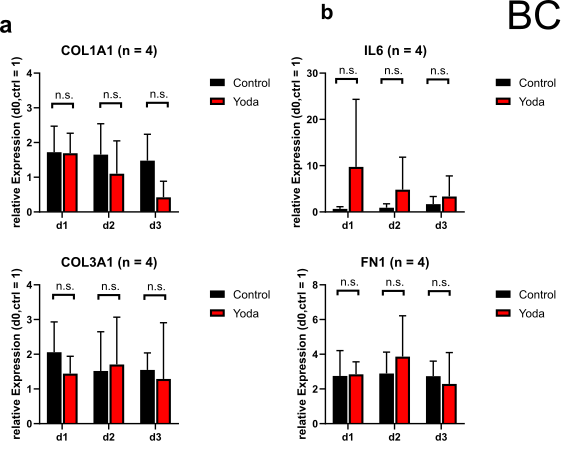
\includegraphics[width = 0.7\textwidth]{NormalYodaExp_PCR.png}
\caption{mRNA levels of selected gene products after 30min chemical stimulation of \Piezo{}, harvested after 24, 48 or 72 hours, denoted by d1, d2 or d3, respectively. Normalized against d0, control.\hfill \newline
\textbf{a.)}: \colone{}
\textbf{b.)}: IL-6
\textbf{c.)}: \colthree{}
\textbf{d.)}: \textsc{Fn}1. 
(Student's t-test with Holm-Sidak multiple comparison correction, n = 4). 
}
\label{fig:Yoda_Norm_PCR}
\end{figure}


\begin{figure}[htbp]
\centering
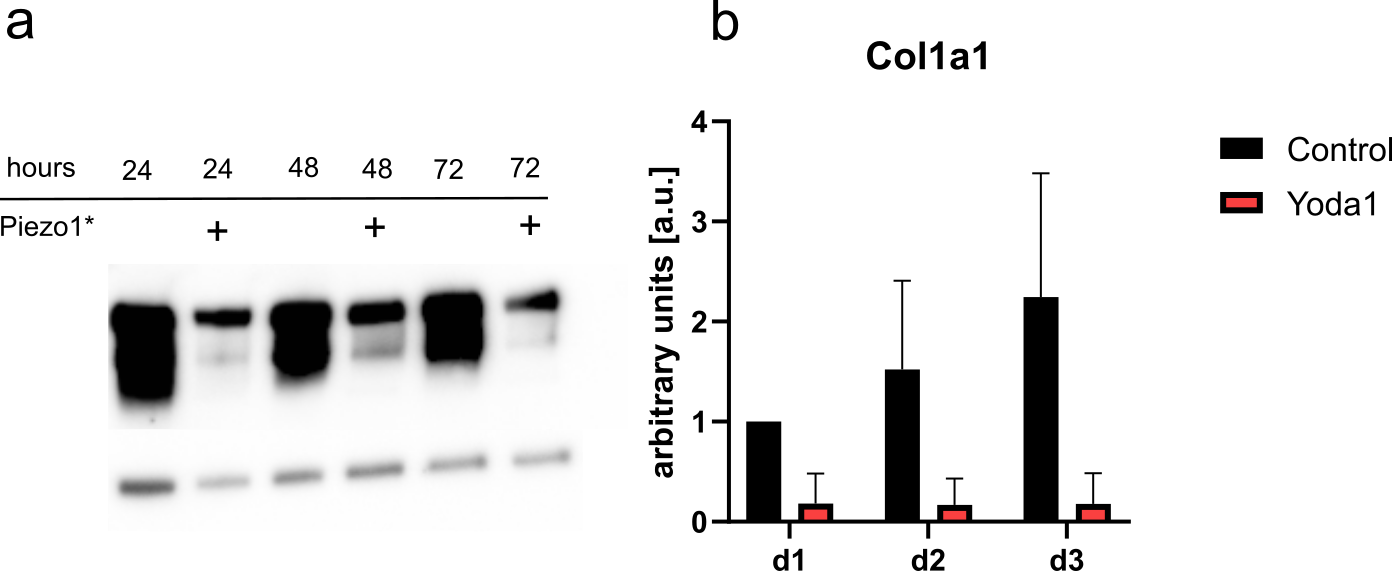
\includegraphics[width = 0.7\textwidth]{NormalYodaExp_WesternBlot_Col1a1.png}
\caption{
\textbf{a.)} Representative Chemiluminescence for \colone with control and chemically stimulated \Piezo{}-samples with alpha-Tubulin as housekeeper.
\textbf{b.)} Quantification of repeated experiments, each data point normalized against housekeeping protein (loading correction) and corresponding d1, control-sample (donor-specific correction).}
\label{fig:Yoda_Norm_WB}
\end{figure}

\section{Reversibility and osteogenic differentiation}
As we saw that intracellular \colone{} remained low on the protein level and was decreasing on the RNA level at the end of our experimental time frame, we wanted to investigate whether the cells would be able to recover and reach a pre-intervention homeostatic state eventually. For this reason, we decided to repeat the experiment from before, but only harvesting the cells after seven days (168 hours). Because in the experiment before we saw qualitatively a steady decrease in cell viability exhibited by morphological changes in \Yoda{}-treated samples\myworries{input figure reference}, we adapted the protocol. In order to allow for sufficient cell survival  until we would harvest the cell for analysis, we changed the medium three days after the intervention. Half of the cells received serum-free MEM\textalpha{} (denoted by S-), whereas the other half was administered MEM\textalpha{} with 10\% FBS (denoted by S+).\\
Interestingly, in our experiment the RNA levels of \colone{} was still drastically lowered independent from FBS supplementation, with as low as 12\% in the serum-starved group  when comparing the \Yoda{} to control sample, both from day 7. While \colthree{} was also low, it is important to note the great variance of \colthree{} expression in the experiment before \myworries{Enter reference}, only allowing limited gain of information at best. IL-6 and \textsc{Fn}1 was slightly reduced. However, due to the experiment being a single measurement, there is only very limited knowledge gain in this experiment. 

\begin{itemize}
\item RNA levels don't differ too much between serum-supplementation groups. Cell Viability and Multiplication however is greatly increased in Serum+ - samples, which is also reflected in the RNA yield size. This way we could accommodate longer experimental time frames, since relaxation could happen, but we just need to increase our time frame. Additionally, it would allow us to do Western Blots which typically need bigger yields to get a better picture. 
\end{itemize}

One alternative explanation would be that the applied \Yoda{}-stimulus lead to a persistent change and possibly to differentiation. MSCs hold the potential for various lineage choices like adipocyte differentiation differentiation for all sorts of differentiation

\begin{itemize}
\item Mention temporal shift in SPP1 and ALPL, but not RUNX2 (late- rather than early osteogenic markers)
\end{itemize}

\begin{figure}[ht]
\centering
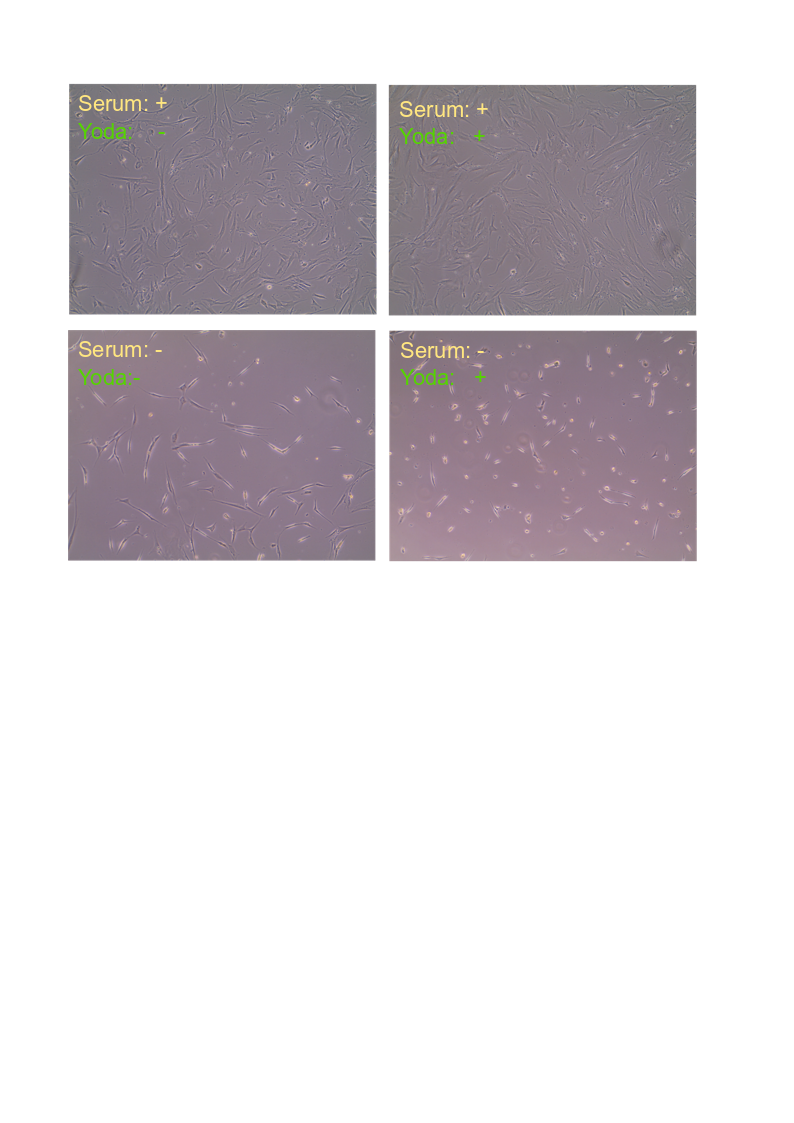
\includegraphics[width = \linewidth{}]{LongTerm_CellPicture.png}
\caption{
Light microscopy picture taken of cells seven days after 30min intervention with either  0\textmu{}M (Yoda: -) or 5\textmu{}M (Yoda: +) chemical \Piezo{}-agonist. Three days after intervention, medium was replaced with either serum-free MEM\textalpha{} (Serum: -) or MEM\textalpha{} supplemented with 10\% FBS (Serum +).}
\label{pic:Cells_LongTerm}
\end{figure}


\begin{figure}
\centering
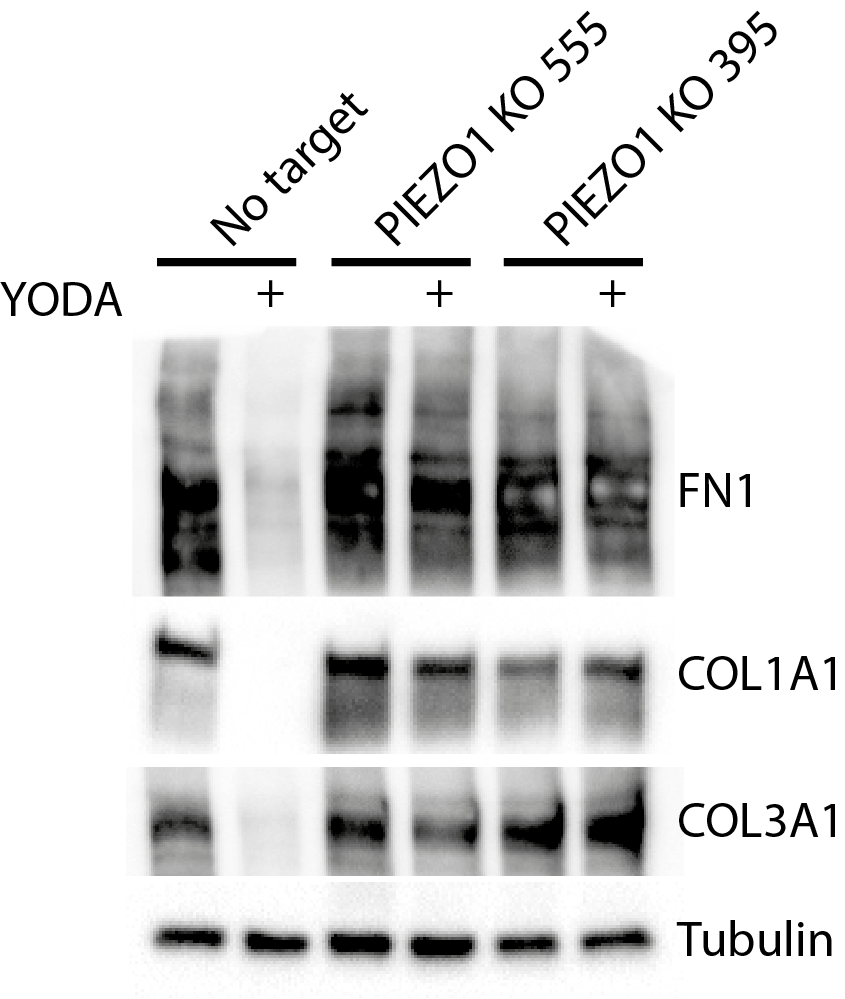
\includegraphics[width=0.7\linewidth]{Uli_Blot_KO.png}
\caption{Western Blot of selected ECM components comparing protein content of different cell lines 3 days after 30min exposure to either MEM\textalpha{} only (negative control) or MEM\textalpha{} supplemented with 5\textmu{}M chemical \Piezo{} agonist (YODA +), \textalpha{}-Tubulin as housekeeping protein. (n=3, Student's t-test)
}
\label{pic:UliBlot}
\end{figure}


\begin{figure}[htbp]
\centering
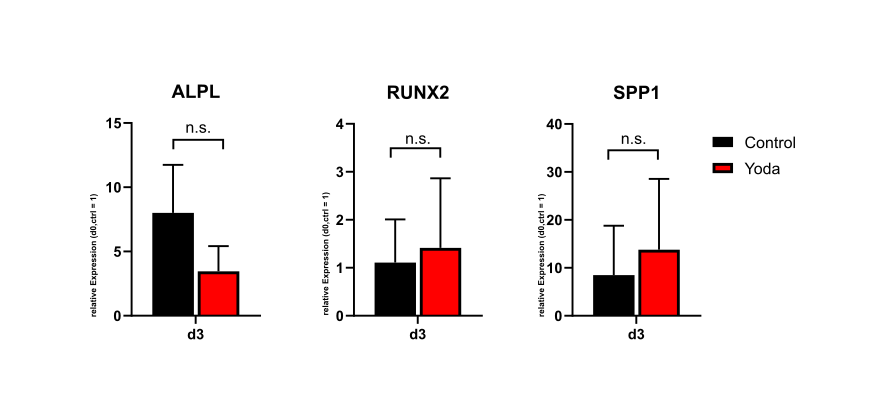
\includegraphics[width = \linewidth]{Osteogenic_PCR_Yoda.png}
\caption{mRNA transcript levels of different late and early osteogenic markers, comparing cells that had underwent 5\textmu{}M \Piezo{} agonist exposure for 30min compared to negative control. (n=3, Student's t-test)}
\label{fig:Long_Term_PCR}
\end{figure}

\begin{figure}
\centering
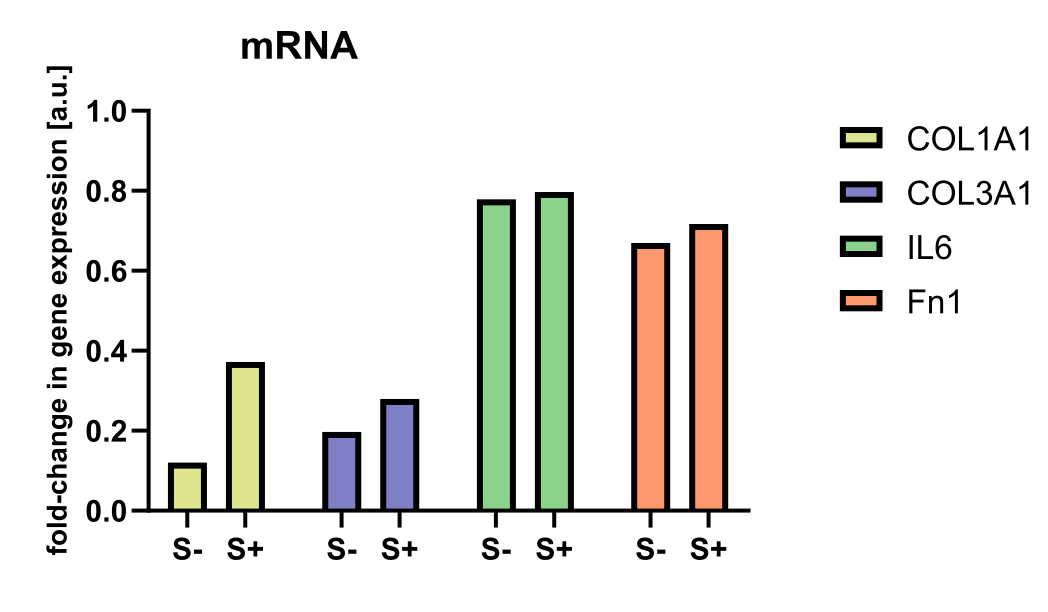
\includegraphics[width = \linewidth{}]{LongTerm_PCR.png}
\caption{mRNA transcript levels of samples that have been harvested seven days after 30min 5\textmu{}M Yoda exposure normalized against corresponding negative control also from seven days post intervention. We changed the media three days after \Yoda intervention and supplemented the MEM\textalpha{} with either 0\% (Serum -) or 10\% FBS (Serum +). (n = 1)}
\label{fig:LongTerm_PCR}
\end{figure}

\section{Excursion: Biostability of Yoda1 and Piezo1 mediated apoptosis}
\label{sec:biostability}
We realised that 3 days after the intervention, there was a large decrease in cell count in Yoda1-treated cells when compared to negative control (see \ref{pic:Yoda_Apop}). Next to Piezo1 being implicated in this pro-apoptotic effect, an intrinsic cytotoxicity of Yoda1 could also be an explanation. To test this hypothesis, Uli, in an explorative experiment, exposed both Piezo1-KO and NoT Cell Lines to Yoda1, which showed that the apoptotic effect is dependent on Piezo1 Expression. (Not shown)

\begin{figure}
\centering
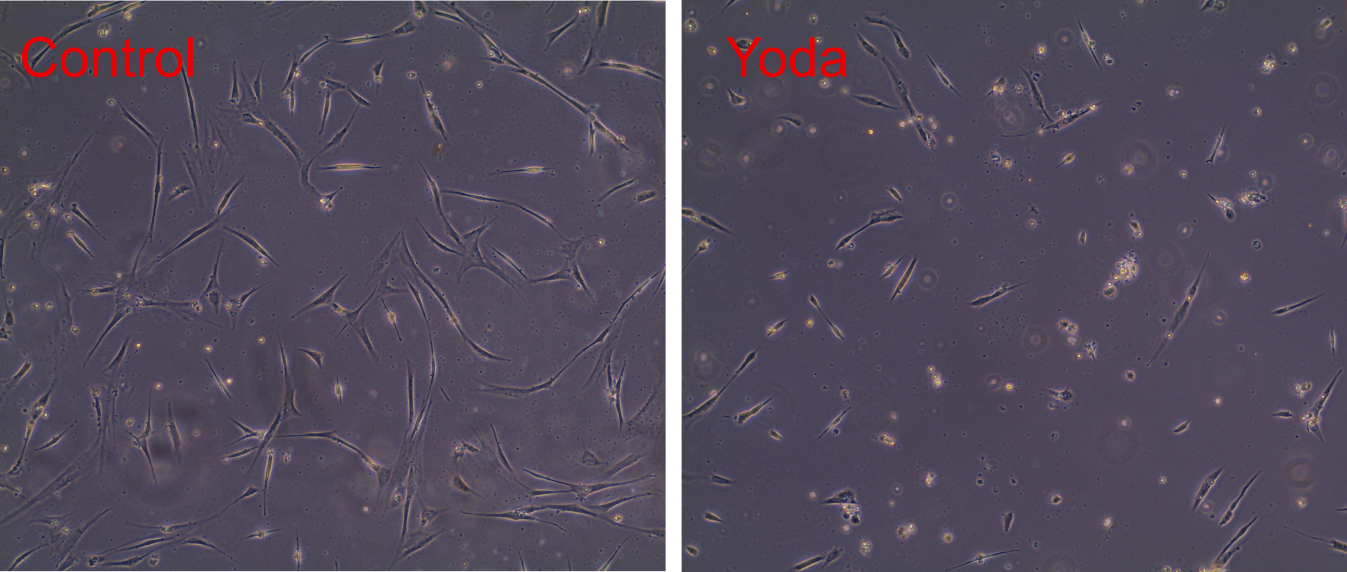
\includegraphics[width = \linewidth]{Yoda_Apoptosis.png}
\caption{Light microscopy picture of serum-starved cells 7 days after intervention with either 0\textmu{}M (negative Control) or 5\textmu{}M (Yoda) chemical \Piezo{}-agonist.}
\label{pic:Yoda_Apop}
\end{figure}